%!TEX TS-program = xelatex
\documentclass[conference]{IEEEtran}
\usepackage[fontset=founder]{ctex} % 增加中文格式的支持。
%\usepackage[fontset=founder,11pt]{ctex} % 小字体,紧凑一点。
\linespread{1.2}
\usepackage{times}

\usepackage[numbers]{natbib}
\usepackage{multicol}
\usepackage[xetex,bookmarks=true]{hyperref}

%\usepackage{cite}

\usepackage[xetex]{graphicx}
\usepackage[cmex10]{amsmath}
\usepackage{amssymb}
\usepackage{import}
\usepackage{bm}

\usepackage{color}
\usepackage{units}
\usepackage{url}
\usepackage{float}
\usepackage{epstopdf}
\usepackage{stmaryrd}

\usepackage{units}
\usepackage{siunitx}

\usepackage{mathtools}

\newcommand{\half}{\ensuremath{\frac{1}{2}}}
\newcommand{\norm}[1]{\left\| #1 \right\|}

%bold-face vectors: maybe they're clearer
\newcommand{\mvec}[1]{\boldsymbol{#1}}
\newcommand{\mvecd}[1]{\dot{\boldsymbol{#1}}}
\newcommand{\mvecdd}[1]{\ddot{\boldsymbol{#1}}}

%matrices: (MATrix SYMbol)
\newcommand{\matSym}[1]{\boldsymbol{#1}}

\newcommand{\mmat}[1]{\begin{bmatrix} #1 \end{bmatrix} }

\newcommand{\msum}[3]{\displaystyle\sum\limits_{#1}^{#2} {#3}}
\newcommand{\mint}[4]{\ensuremath{\displaystyle\int\limits_{#1}^{#2} \! {#3} \, {#4} }}

\newcommand{\mrb}[1]{\left( #1 \right)} %enclose in round brackets
\newcommand{\msb}[1]{\left[ #1 \right]} %enclose in square brackets
\newcommand{\mcb}[1]{\left\{ #1 \right\}} %enclose in curly brackets
\newcommand{\mabs}[1]{\left| #1 \right|} %enclose in | . |

\newcommand{\todo}[1]{\textcolor{red}{TODO: #1}}
\newcommand{\commentOut}[1]{}

\newcommand{\figref}[1]{Fig.~\ref{#1}}
\newcommand{\secref}[1]{Section~\ref{#1}}
%\newcommand{\eqref}[1]{(\ref{#1})}

\newcommand{\realNums}{\ensuremath{\mathbb{R}}}
\newcommand{\skewSym}[1]{\ensuremath{\,S\!\mrb{#1}}}
\newcommand{\skewSymInv}[1]{\ensuremath{\,{v}\!\mrb{#1}}}

\newcommand{\trace}[1]{\ensuremath{\mathrm{tr}\!\mrb{#1}}}
\newcommand{\diag}[1]{\ensuremath{\mathrm{diag}\!\mrb{#1}}}

\newcommand{\SOthree}{\ensuremath{\mathrm{SO}\mrb{3}}}
\newcommand{\sothree}{\ensuremath{\mathrm{so}\mrb{3}}}

%%%%%%%%%%%%%%%%%


\newcommand{\ddt}{\ensuremath{\frac{\mathrm{d}}{\mathrm{d}t}}}
\newcommand{\ddtSq}{\ensuremath{\frac{\mathrm{d}^2}{\mathrm{d}t^2}}}

\newcommand{\identityMat }{\ensuremath{\mvec{I}}}

\newcommand{\rotMat}{\ensuremath{\mvec{R}}}
\newcommand{\rotAngle}{\ensuremath{\rho}}
\newcommand{\rotAxis}{\ensuremath{\mvec{n}}}

\newcommand{\rotAngleErr}{\ensuremath{\rho}_\mathrm{e}}
\newcommand{\rotAxisErr}{\ensuremath{\mvec{n}_\mathrm{e}}}

\newcommand{\rotMatDes}{\ensuremath{\mvec{R}_\mathrm{des}}}
\newcommand{\rotMatErr}{\ensuremath{\mvec{R}_\mathrm{e}}}

\newcommand{\rotMatReduced}{\ensuremath{\mvec{R}_r}}
\newcommand{\rotMatYaw}{\ensuremath{\mvec{R}_y}}
\newcommand{\rotAngleReduced}{\ensuremath{\rho_r}}
\newcommand{\rotAxisReduced}{\ensuremath{\mvec{n}_r}}
\newcommand{\rotAngleYaw}{\ensuremath{\rho_y}}
\newcommand{\rotAxisYaw}{\ensuremath{\mvec{n}_y}}

\newcommand{\baseVec}[1]{\ensuremath{\mvec{e}_{#1}}}

\newcommand{\angVel}{\ensuremath{\mvec{\omega}}}
\newcommand{\angVelDes}{\ensuremath{\mvec{\omega}_\mathrm{des}}}
\newcommand{\angVelErr}{\ensuremath{\mvec{\omega}_\mathrm{e}}}

\newcommand{\angAcc}{\ensuremath{\mvec{\alpha}}}
\newcommand{\angAccDes}{\ensuremath{\mvec{\alpha}_\mathrm{des}}}
\newcommand{\angAccErr}{\ensuremath{\mvec{\alpha}_\mathrm{e}}}

\newcommand{\pos}{\ensuremath{\mvec{p}}}
\newcommand{\posDes}{\ensuremath{\mvec{p}_\mathrm{des}}}
\newcommand{\translAccDes}{\ensuremath{\mvec{a}_\mathrm{des}}}

\newcommand{\translAcc}{\ensuremath{\mvec{a}}}
\newcommand{\thrustDir}{\ensuremath{\baseVec{3}}}
\newcommand{\gravity}{\ensuremath{\mvec{g}}}
\newcommand{\mass}{\ensuremath{m}}
\newcommand{\thrustMag}{\ensuremath{f_\Sigma}}
\newcommand{\thrustMagDes}{\ensuremath{f_{\Sigma,\mathrm{des}}}}
\newcommand{\mmoi}{\ensuremath{\mvec{J}}}
\newcommand{\moments}{\ensuremath{\mvec{\tau}}}

\newcommand{\angAccInpSS}{\ensuremath{\mvec{\alpha}_\mathrm{e,des}^\mathrm{SS}}}
\newcommand{\angAccInpRV}{\ensuremath{\mvec{\alpha}_\mathrm{e,des}^\mathrm{RV}}}
\newcommand{\angAccInpTP}{\ensuremath{\mvec{\alpha}_\mathrm{e,des}^\mathrm{QTP}}}
\newcommand{\angAccInpNEW}{\ensuremath{\mvec{\alpha}_\mathrm{e,des}^\mathrm{New}}}

\newcommand{\lyapFnSS}{\ensuremath{J^\mathrm{SS}}}
\newcommand{\lyapFnRV}{\ensuremath{J^\mathrm{RV}}}
\newcommand{\lyapFnTP}{\ensuremath{J^\mathrm{QTP}}}
\newcommand{\lyapFnNEW}{\ensuremath{J^\mathrm{New}}}

\newcommand{\gainAtt}{\ensuremath{K_{R}}}
\newcommand{\gainRates}{\ensuremath{K_\omega}}

\newcommand{\gainPos}{\ensuremath{k_{p}}}
\newcommand{\gainVel}{\ensuremath{k_{\dot{p}}}}

\newcommand{\gainAttRed}{\ensuremath{k_{r}}}
\newcommand{\gainAttYaw}{\ensuremath{k_{y}}}



\title{\LARGE \bf
用于从大的干扰中恢复的多旋翼姿态控制
}

\author{
%Author Names Omitted for Anonymous Review. Paper-ID 44
Mark W. Mueller% <-this % stops a space
\thanks{The author is with the Mechanical Engineering Department, UC Berkeley.
\newline        {\tt\small mwm@berkeley.edu}}%
}

\begin{document}

\maketitle
\thispagestyle{empty}
\pagestyle{empty}

%%%%%%%%%%%%%%%%%%%%%%%%%%%%%%%%%%%%%%%%%%%%%%%%%%%%%%%%%%%%%%%%%%%%%%%%%%%%%%%%
\begin{abstract}

我们提出了一种新颖的、高性能的多旋翼姿态控制律,以期从大干扰中恢复。该控制器与文献中三种成熟的替代方案进行了比较。所考虑的所有控制器在一阶上都是相同的,但在姿态误差计算上有所不同。我们表明,从安全角度来看,普遍使用的旋转矩阵的斜对称部分是有问题的,特别是闭环系统可能会在大的姿态误差下停留任意时间(这将导致实际系统的潜在故障)。新提出的控制器优先考虑飞行器推力方向上的误差,其性能优于文献中类似的现有控制器。稳定性通过Lyapunov函数实现,控制器在实验中得到验证。这种新型控制器在安全关键情况下尤其具有吸引力,在这种情况下,多旋翼可能需要从大的初始干扰中恢复。

\end{abstract}

% !TEX root = micro_Lie_theory.tex

\section{序言}
\label{sec:intro}

在过去的几年里,机器人业界做出了巨大的努力来正确地用方程式确切表达估计问题。 
这是由于人们对方程解的精确性、一致性和稳定性的要求越来越高。 
事实上,对状态和测量、相关函数及其不确定性的适当建模对于实现这些目标至关重要。
这导致了涉及所谓“流形”的设计,在这种情况下,流形不亚于Lie群的光滑拓扑表面,这是状态表示的演化。
借助于Lie理论(Lie theory, LT),我们可以构造一个严格的微积分文献,精确而容易地处理不确定性、导数和积分。
通常,这些工作都集中在众所周知的旋转流形 $\SO(3)$ 和刚体运动 $\SE(3)$。

\begin{figure}[tb]
\centering
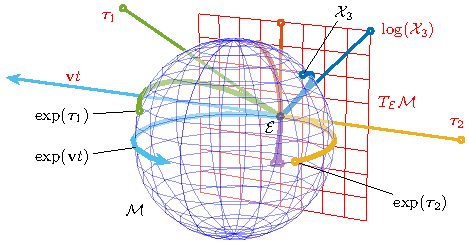
\includegraphics{figures/exponential}
\caption{Lie群与Lie代数关系的表示。
Lie代数 $\mtanat{\cM}{\cE}$ (红色平面)是Lie群流形 $\cM$ (这里用蓝色球面表示)在幺元 $\cE$ 处的切空间。
通过指数映射,每个通过Lie代数原点的直接路径 $\bfv t$ 产生一个围绕流形的路径 $\exp(\bfv t)$ ,流形沿着各自的测地线运行。 
相反的,群中的每个元素在李代数中都有一个等价项。
这种关系是如此深刻,以至于(几乎)群中的所有运算,那些曲线的和非线性的,在李代数中,这是一个线性向量空间,有一个精确的等价。
虽然 $\bbR^3$ 中的球面不是Lie群(我们只是把它当作一个可以画在纸上的表示),但 $\bbR^4$ 中的球面是Lie群,它描述了单位四元数群 --- 参见 \figRef{fig:manifold_q} 和 \exRef{ex:S3} 。
}
\label{fig:exponential}
\end{figure}

当第一次介绍Lie群时,从不同的角度看待它是很重要的。 
拓扑观点,参见 \figRef{fig:exponential} ,涉及流形的形状,并传达其与切空间和指数映射关系的强大直觉。
代数观点涉及群运算及其具体实现,允许利用代数性质来扩展闭式公式或简化它们。
几何视点在机器人学中特别有用,它将群元素与机体或参考坐标系中的位置、速度、方向和/或其它改变相关联。
原始坐标系可以用群的幺元来标识,并且流形上的任意其它点表示某个“局部”坐标系。
借助这些类比,Lie理论的许多数学抽象可以更接近向量空间、几何、运动学和其它更经典领域的直观概念。


Lie理论绝不简单。 
为了掌握Lie理论的最小概念,我们可以参考下面的三个参考文献。 
首先,Abbaspour的 \emph{``Basic Lie theory"}~\cite{ABBASPOUR-2007-Basic_Lie_theory} 有400多页。
也是类似的标题,Howe的 \emph{``Very basic Lie theory"}~\cite{Howe-Basic_Lie} 共有24(稠密的)页,有时被认为是必读的介绍。
最后,更现代、更著名的Stillwell的 \emph{``Naive Lie theory"}~\cite{STILLWELL-08} 共有200多页。
%
由于这些先例被标记为“基本的”、“非常基本的”和“幼稚的”,本文仅 \pageref{LastPage} 页的目的是进一步简化Lie理论 (因此标题中的形容词为 `微型(micro)')。
我们用两种方式来做。
首先,我们从Lie理论中选择一个素材的小子集。这个子集如此之小,以至于它仅仅是探索Lie理论的潜力。 
然而,它对于我们在机器人学中处理的估计问题(例如惯性预积分、里程计和SLAM、视觉伺服等)中的不确定性管理似乎非常有用,从而实现优化的优雅和严格的设计。
第二,我们用教学的方式来解释它,用大量的冗余来减少进入Lie理论的鸿沟,我们认为这仍然是必需的。
也就是说,我们坚持朝着这个方向努力,命名一个范例标题,Stillwell的文献 \cite{STILLWELL-08},并提供一个更简化的版本。
虽然我们试图将抽象级别保持在最低限度,但正文主体是通用的。
当应用到已知的群(旋转和运动矩阵、四元数等)时,插入的示例作为一般概念的基础。 
此外,许多标题非常冗长的插图再次解释了相同的概念。
我们特别关注Jacobian矩阵的计算 (这是一个在文献 \cite{STILLWELL-08} 中没有讨论的主题),它是大多数优化算法的关键,也是设计新算法时的麻烦源。
我们在最后一章给出了机器人定位和映射的应用实例,并在Lie理论基础上实现了EKF和非线性优化算法。
最后,几个附录包含了机器人学中最常用群最相关的详细信息:单位复数、四元数、二维和三维旋转矩阵、二维和三维刚体运动矩阵以及平凡平移群。


然而,我们对Lie理论最重要的简化是在范围方面。 
下面来自 
Howe~\cite{Howe-Basic_Lie} 的一段话可以帮助我们说明我们留下的东西:
%
``\emph{Lie理论的本质现象是人们可以用一种自然的方式联想到Lie群 $\cG$ 和它的Lie代数 $\frak{g}$。
Lie代数 $\frak{g}$ 首先是一个向量空间,其次被赋予一个称为Lie括号 [...] 的双线性非关联积。 
令人惊奇的是,群 $\cG$ 几乎完全由 $\frak{g}$ 和它的Lie括号决定。
因此,对于许多用途,可以用 $\frak{g}$ 代替 $\cG$。
因为 $\cG$ 是一个复杂的非线性对象,而 $\frak{g}$ 只是一个向量空间,所以使用 $\frak{g}$ 通常非常简单。
[...] 
这是Lie理论的力量源泉之一。%
}"
%
在文献 \cite{STILLWELL-08},Stillwell 甚至称为 ``\emph{Lie理论的奇迹}''.
在本次工作中,我们将有效地将Lie代数降级到第二平面,以支持它的等价向量空间 $\bbR^n$,因而根本不引入Lie括号。
因此,Lie群和它的Lie代数之间的联系在这里将不会像它应有的那样深刻。
我们的立场是,鉴于我们所预见的目标应用领域,这种(包含Lie括号的)素材通常是没有必要的。
%). 
此外,如果包含Lie括号在内,那么我们将无法达到清晰和有用的目标,因为读者将不得不进入数学概念,这些概念由于其抽象性或微妙性而变得不必要的复杂。



我们的努力与最近关于这个主题 ~\cite{BARFOOT-17-Estimation,EADE-Lie,forster2017-TRO} 的其它工作是一致的,这些工作也显示了带入Lie理论更进入机器人的需求。
我们的方法旨在让本文的目标读者,熟悉状态估计(Kalman滤波、基于图的优化等),但还不熟悉Lie理论的理论文献的读者,熟悉该理论。
%
为此,我们在符号方面采取了一些倡议,特别是在导数的定义方面,使其接近向量对应项,从而使链式规则清晰可见。
如前所述,我们实际上选择了避免Lie代数的素材,而是更喜欢研究它的同构切向量空间 $\bbR^n$,这是我们最终表示不确定性或(小)状态增量的地方。
所有这些步骤都是在绝对没有精度或准确性损失的情况下进行的,我们相信它们使得理解Lie理论及其工具的操作更容易。

本文伴随一个新的开源的只有头文件的 C++ 代码库,称为 \manif\ \cite{DERAY-20-manif},可以在这里找到: \url{https://github.com/artivis/manif} 。
\manif\ 实现广泛使用的群 $\SO(2)$, $\SO(3)$, $\SE(2)$ 和 $\SE(3)$,并支持创建分析 Jacobian 矩阵。
该库为易于使用、灵活性和性能而设计。

 
\section{问题描述}
\label{secDynamics}

传统的多翼机的特点是具有偶数个(至少四个)大小相等的固定螺距螺旋桨,这些螺旋桨围绕几何中心以旋转对称的方式排列,几何中心大致与飞行器的电池、电子设备和有效载荷重合。 
螺旋桨手性交替排列,以便使它们的空气动力学的反应扭矩的总和为零。 

除了这种典型的配置外,许多其它的设计也是可能的,并且已经被考虑过。 
例如,使用直径大不相同的螺旋桨以提高效率 \cite{pounds2002design},使螺旋桨可倾斜 \cite{ryll2012modeling},以及螺旋桨不对齐的飞行器,使其平移能力被完全激励 \cite{mehmood2016maneuverability}。
尽管这类飞行器并不完全符合下面的描述,但它们的姿态控制问题是相似的,因为它们能够产生任意的3D扭矩,因此它们的姿态动力学是被完全激励的。
%There are, however, multicopter designs where the attitude dynamics are not fully actuated, see e.g. \cite{mueller2015relaxed,zhang2016controllable}.

\subsection{动力学}

\begin{figure}
  \centering
  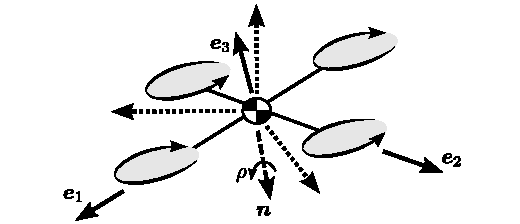
\includegraphics{Figures/quadcopter.pdf}
  \caption{
  一架多旋翼飞机带机体固连轴 $\baseVec{1}$、$\baseVec{2}$ 和 $\baseVec{3}$,从点线表示的期望的轴,被 $\rotMat$ 旋转过来。
  旋转 $\rotMat$ 是围绕单位向量 $\rotAxis$,角度为 $\rotAngle$ 的旋转。
  }
  \label{figModel}
\end{figure}

多旋翼飞机的方向(将机体固连坐标系与惯性坐标系联系起来)由旋转矩阵 $\rotMat\in\SOthree$ 描述,而角速度由 $\angVel\in\realNums^3$ 给出。 
旋转矩阵主要通过推力向量的方向来影响多旋翼飞机的运动,推力向量相对于飞行器有固定方向。

飞行器的螺旋桨都在相同的机体固连方向上产生推力 $\thrustDir$,并且量值为 $\thrustMag$,示意图参见 \figref{figModel}。
飞行器具有质量 $\mass$,受到重力加速度 $\gravity$ 的作用,因此,飞行器平移加速度 $\translAcc$ 给出为 
\begin{align}
	\translAcc = \frac{1}{\mass} \rotMat \thrustDir \thrustMag + \gravity. \label{eqDynamicsTranslAcc}
\end{align}
因此,通过控制飞行器的姿态和指定总推力,可以控制平移加速度。
从方程 \eqref{eqDynamicsTranslAcc} 中值得注意的是,姿态的三个自由度中只有两个与平移动力学有关,特别是围绕飞行器的 $\baseVec{3}$ 轴的旋转并不重要。 

姿态演变为 
\begin{align}
	\dot{\rotMat} = \rotMat \skewSym{\angVel}
\end{align}
其中 $\skewSym{\cdot}: \realNums^3\rightarrow\sothree$ 产生向量参数的倾斜对称矩阵形式 (通常称为 ``hat-map''),特别是如果 $\mvec{x}=\mrb{x_1, x_2, x_3}$ 则 
\begin{align}
	\skewSym{\mvec{x}} = \mmat{0 & -x_3 & x_2\\ x_3 & 0 & -x_1 \\ -x_2 & x_1 & 0}
\end{align}
值得注意的是,对于 $\mvec{x},\mvec{y}\in\realNums^3$ 以及 $\rotMat\in\SOthree$ \cite{bernstein2009matrix}
\begin{align}
  \skewSym{\mvec{x}} &= -\skewSym{\mvec{x}}^T
\\\skewSym{\mvec{x}}\mvec{y} &= \mvec{x}\times\mvec{y} = -\skewSym{\mvec{y}}\mvec{x}
\\\skewSym{\rotMat\mvec{x}} &= \rotMat\skewSym{\mvec{x}} \rotMat^T
\end{align}
上述 $\skewSym{\cdot}$ 的逆函数是 $\skewSymInv{\cdot}:\sothree\rightarrow\realNums^3$,所以
\begin{align}
	\skewSymInv{\skewSym{\mvec{x}}} = \mvec{x}
\end{align}

角加速度 $\angAcc$ 是飞行器质量惯性矩张量 $\mmoi$、作用在飞行器上的外部力矩 $\moments$ 和当前角速度的函数,为 
\begin{align}
	\angAcc = \dot{\angVel} = \mmoi^{-1}\mrb{\moments - \skewSym{\angVel}\mmoi\angVel} \label{eqDynamicsAngAcc}
\end{align}

所有传统多旋翼飞机(四旋翼、六旋翼和八旋翼)的配置都可以使飞行器产生一个任意(达到电机力饱和)的三维力矩 $\moments$,其与总推力 $\thrustMag$无关。
作为单个螺旋桨力的函数,力矩和总推力的计算以直截了当的方式遵循飞行器的几何形状和螺旋桨的特性。
典型的多旋翼飞机的一个重要特征是,它们能够在垂直于推力向量的方向上产生比围绕推力向量大得多的扭矩。
这是由于螺旋桨与质心的距离很大,这可能比螺旋桨的空气动力扭矩与推力的比率大一个数量级以上。 
对于敏捷机动在计算推力方面的深入讨论,示例参见文献 \cite{faessler2017thrust}。

\subsection{控制问题}
因此,从方程 \eqref{eqDynamicsAngAcc} 可以看出,在任何瞬时角速度下都可以产生任意的角加速度 $\angAcc$ (直至电机推力饱和)。
这促使将角加速度用作姿态子系统的控制输入,并且特别的是,这意味着多旋翼飞机的姿态可以被视为被完全激励,从而得到更简单的姿态动力学:
\begin{align}
	\dot{\rotMat} &= \rotMat\skewSym{\angVel}
\\	\dot{\angVel} &= \angAcc
\end{align}

我们认为控制问题是将飞行器的方向控制在一个期望的姿态 $\rotMatDes$,它有一个相关的期望的角速度 $\angVelDes$ 和角加速度 $\angAccDes$,以便 
\begin{align}
	\ddt\rotMatDes =& \rotMatDes \skewSym{\angVelDes}
\\  \ddt \angVelDes =& \angAccDes
\end{align}
旋转误差 $\rotMatErr$ 和它的角速度 $\angVelErr$ 被定义为 
\begin{align}
	\rotMatErr =& \rotMatDes^{-1} \rotMat \label{eqDefineRotMatErr}
\\  \ddt \rotMatErr =& \rotMatErr \skewSym{\angVelErr} \label{eqDefineAngVelErr}
\end{align}

代入旋转误差的定义,并经过一些代数运算,由此得出 
\begin{align}
  \angVelErr &= \angVel - \rotMatErr^{-1} \angVelDes
\\ \angAccErr &= \ddt \angVelErr = \angAcc - \rotMatErr^{-1} \angAccDes + \skewSym{\angVelErr} \angVelDes \label{eqDefAngAccErr}
\end{align}

为紧凑起见,我们将使用 $\angAccErr$ 作为控制输入,注意,指令扭矩是通过将方程 \eqref{eqDefAngAccErr} 代入方程 \eqref{eqDynamicsAngAcc} 恢复的。

为了进行分析,通常更直观的方法是将旋转矩阵 $\rotMat$ 表示为旋转向量,其被分解为角度 $\rotAngle\in[0,\pi]$ 和单位长度旋转轴 $\rotAxis$ (通常称为特征轴)。
这些数量之间的关系由文献 \cite{shuster1993survey} 给出为 
\begin{align}
	\rotMat = \cos\rotAngle\identityMat + \mrb{1-\cos\rotAngle}\rotAxis\rotAxis^T + \sin\rotAngle\skewSym{\rotAxis}
	\label{eqRotMatFromAxisAngle}
\end{align}
由此,给定旋转矩阵的角度和轴也可以直接向前恢复,除非以 $180^\circ$ 的旋转,此时围绕 $\rotAxis$ 和 $-\rotAxis$ 的旋转是相同的,以及与轴不相关的零旋转。







 
\section{控制器}
\label{secControllers}

我们考虑了四种不同的控制布局,其中三种在有趣和具有挑战性的环境中都有过应用历史,而第四种是一种新的算法。
所有的控制器都有一个与角速度成比例的动作,以及一个与飞行器姿态(以某种表示)成比例的动作分量。
 这些控制器的主要区别在于该姿态的表示,并且尽管这些控制器在一阶上是相同的,但在下一节中会显示,对于大的姿态误差会出现重要的差异。

\subsection{斜对称控制}

这种控制如文献 \cite{lee2010geometric} 所述,并且首先提出它是因为它在文献中的使用特别广泛(有一些示例包括文献 \cite{sreenath2013geometric,goodarzi2013geometric,lee2013nonlinear,simha2017almost,rashad2017design}),特别是它在有影响力的文献 \cite{mahony2012aerial} 中的使用。
注意,我们使用了一个大大不同的符号和表示方法,希望提供一个统一的比较和额外的洞察力。

姿态误差由旋转矩阵的斜对称分量计算出来,因此期望的角加速度给出为 
\begin{align}
	\angAccInpSS := -\gainRates \angVelErr - \half \gainAtt \skewSymInv{\rotMatErr-\rotMatErr^T} \label{eqDefInputSS}
\end{align}
其中 $\gainRates$ 和 $\gainAtt$ 为正定控制器增益,每种增益都是 $\realNums^{3\times3}$。
注意,可以通过方程 \eqref{eqRotMatFromAxisAngle} 重写姿态分量,为 
\begin{align}
	\half \skewSymInv{\rotMatErr-\rotMatErr^T} = \sin \rotAngleErr\, \rotAxisErr
\end{align}
因此
\begin{align}
	\angAccInpSS = -\gainRates \angVelErr - \gainAtt \sin\rotAngleErr\, \rotAxisErr.\label{eqSkewSymmControllerAxAngle}
\end{align}

该控制器的稳定性可以用下面的 Lyapunov 函数来研究 
\begin{align}
	\lyapFnSS := \frac{1}{2} \angVelErr^T \gainAtt^{-1} \angVelErr + \frac{3 - \trace{\rotMatErr}}{2}
\end{align}
其中,矩阵的迹 $\trace{\rotMatErr}$ 与旋转角度相关,如下所示 
\begin{align}
	\trace{\rotMatErr} =& \msum{i=1}{3}{\baseVec{i}^T\rotMatErr\baseVec{i}} \label{eqRotTraceBaseVectors}
\\ =& 2\cos{\rotAngleErr} + 1
\end{align}
其中后面的等式来自于方程 \eqref{eqRotMatFromAxisAngle}。 
因此,Lyapunov 函数可以更直观地写为 
\begin{align}
	\lyapFnSS := \half \angVelErr^T \gainAtt^{-1} \angVelErr + \mrb{1-\cos\rotAngleErr}
\end{align}
我们可以很容易地验证它是一个有效的候选 Lyapunov 函数。 

矩阵的迹 $\trace{\rotMatErr}$ 的时间导数从方程 \eqref{eqRotTraceBaseVectors} 得出为 
\begin{align}
	\ddt \trace{\rotMatErr} =& 
	%\msum{i=1}{3}{\baseVec{i}^T  \rotMatErr \skewSym{\angVelErr} \baseVec{i}} =
	 -\msum{i=1}{3}{\baseVec{i}^T  \rotMatErr \skewSym{\baseVec{i}} \angVelErr}.
\end{align}
此外,通过直接计算,它可以被证明为  
%see ``test.py'' script
\begin{align}
  \msum{i=1}{3}{\baseVec{i}^T  \rotMatErr \skewSym{\baseVec{i}} } = \skewSymInv{\rotMatErr-\rotMatErr^T}^T
\end{align}

因此,取 Lyapunov 函数的时间导数以获得 
\begin{align}
	\ddt \lyapFnSS =& \angVelErr^T\mrb{\gainAtt^{-1} \angAcc + \half \skewSymInv{\rotMatErr-\rotMatErr^T}}
%\\=& \angVelErr^T\mrb{-\gainAtt^{-1}\gainRates \angVelErr - \mrb{\gainAtt^{-1} \gainAtt-\identityMat} \skewSymInv{\rotMatErr-\rotMatErr^T} }
\\=& -\angVelErr^T \gainAtt^{-1}\gainRates \angVelErr \leq 0
\end{align}
通过注意二阶时间导数,渐进稳定性给出为 
\begin{align}
\begin{split}
	\ddtSq \lyapFnSS=& \angVelErr^T \mrb{\gainAtt^{-1}\gainRates + \gainRates^T\gainAtt^{-T}}\cdot
	\\ & \mrb{-\gainAtt \sin\rotAngleErr\rotAxisErr - \gainRates \angVelErr }
\end{split}
\end{align}
负半定导数意味着 $\lyapFnSS(t)\leq\lyapFnSS(0)$;反过来形成角速度 $\angVelErr$ 的界限。
从这个界限来看,二阶导数是有界限的,所以 $\ddt\lyapFnSS$ 是一致连续和可积的。 
因此,当 $t\rightarrow\infty$ 时,根据 Barbalat 引理,$\ddt\lyapFnSS \rightarrow 0$,并且明确地, $\angVelErr\rightarrow0$。 
代入控制法可以得出结论,如果 $\rotAngleErr\neq\pi$,则方向误差也会收敛到特征值,从而建立渐近稳定性。

%\todo{Not allowed to LaSalle: So that asymptotic stability follows by invoking LaSalle's principle \cite{sastry2013nonlinear}.}
%\todo{KS: Control in [9] provides exponential stability for a set of rotation errors. Do you want to specialize your development to illustrate this?}

一个非常密切相关的控制策略是用不同的标量值 \cite{chaturvedi2011rigid} 对方程 \eqref{eqRotTraceBaseVectors} 右侧的各项进行加权总和。
由此产生的闭环系统具有一些理想的特性(并且其稳定性在文献 \cite{chaturvedi2011rigid} 中得到了证明,而不依赖于 Lyapunov 函数),并且在姿态动力学中引入了在方程 \eqref{eqDefInputSS} 中不存在的三个鞍点。 
然而,该控制器足够相似,我们只考虑所有项都具有相等权重的更简单形式。


\subsection{旋转向量控制}
对于这种控制策略,使用旋转向量计算姿态误差(以便反馈的姿态部分与角度误差成比例)。
所期望的角加速度为 
\begin{align}
	\angAccInpRV := -\gainRates \angVelErr - \gainAtt \rotAngleErr \, \rotAxisErr \label{eqDefInputRotVec}
\end{align}
其中 $\gainRates$ 和 $\gainAtt$ 同样是正定的增益矩阵。
注意,根据定义,角度是有界限的,因此 $0\leq\rotAngleErr\leq\pi$。
此外,注意与方程 \eqref{eqDefInputSS} 的相似性,关键的区别在于这里使用了角度值,而不是它的正弦值。

利用 Lyapunov 函数分析其所产生的闭环系统的稳定性 
\begin{align}
	\lyapFnRV :=& \half \angVelErr^T \gainAtt^{-1} \angVelErr + \half \mrb{\arccos\frac{\trace{\rotMatErr}-1}{2}}^2 \label{eqLyapRotVec}
\end{align}
其可简化为 
\begin{align}
	\lyapFnRV =  \half \angVelErr^T \gainAtt^{-1} \angVelErr + \half \rotAngleErr^2
\end{align}

注意到旋转角度的时间导数由文献 \cite[方程 (270)]{shuster1993survey} 给出为 
\begin{align}
	\ddt \rotAngleErr = \rotAxisErr^T \angVelErr \label{eqTimeDerivativeRotAngle}
\end{align}
则方程 \eqref{eqLyapRotVec} 的时间导数跟着为 
\begin{align}
	\ddt \lyapFnRV =& \angVelErr^T \gainAtt^{-1} \angAcc + \rotAngleErr \angVelErr^T\rotAxisErr
	\\ =& - \angVelErr^T \gainAtt^{-1} \gainRates \angVelErr  \leq 0
\end{align}
从这一点来看,通过注意到有界限的二阶导数并援引 Barbalat 引理,渐近稳定性与斜对称控制器类似。 
同样,这需要 $\rotAngleErr\neq\pi$。
%\todo{Not allowed to use LaSalle's principle allowing to conclude asymptotic stability.}
%\todo{Also, talk about the advantages\ldots}
%\todo{KS: Do you have exponential stability for $\rotAngle<\pi/2$?}

旋转向量的使用在概念上很优雅,因为控制动作与角度成比例,即使是大的姿态误差也是如此。
这意味着系统的闭环行为(如果限制在一个单一的旋转自由度上)将表现得像一个二阶阻尼系统,即使是大角度,只要 $\rotAngleErr<180^\circ$。
然而,当角度`穿过' $180^\circ$ 时,控制输入会有不连续性,因为对于 $\rotAxisErr$ 的符号会翻转。

\subsection{基于四元数的倾斜优先控制}
这种控制器基于这样的直觉,即四旋翼飞机姿态的最重要部分是其推力轴的方向,因此应优先控制该方向,而不是其它单一的姿态自由度。
该控制器在文献 \cite{brescianini2013nonlinear} 中提出,并且其推导基于旋转四元数。
在这里它被转变为旋转矩阵表示法,以便更好地与其它两种已提出的方法放在相同上下文进行比较,并作为拟议的控制器的预览。

姿态误差被分为两部分:一个优先的`减小的'姿态 $\rotMatReduced$,表示将推力方向与所期望的推力方向对齐的最短旋转,以及一个围绕推力轴的旋转 $\rotMatYaw$,表示围绕推力轴的剩余旋转。
具体地,减小的姿态是最小的旋转,对它来说 
\begin{align}
	\rotMatErr\rotMatReduced^T  \thrustDir =& \thrustDir \label{eqDefRedAtt1}
\end{align}
并且 
\begin{align}
  \rotMatErr  =& \rotMatYaw \rotMatReduced \label{eqDefRedAtt2}
\end{align}
由此可知,$\rotMatYaw$ 是一个纯粹地围绕 $\thrustDir$ 的旋转。
注意,这个角度在一阶上等同于(3-2-1 偏航-俯仰-横滚序列的)欧拉`偏航'角。

与 $\rotMatReduced$ 相对应的轴 $\rotAxisReduced$ 和角度 $\rotAngleReduced$ 可计算为 
\begin{align}
  \rotAngleReduced =& \arccos {\thrustDir^T\rotMatErr\thrustDir} \label{eqComputeReducedRotAngle}
\\\rotAxisReduced =& \frac{\skewSym{\rotMatErr^T\thrustDir}\thrustDir}{\norm{\skewSym{\rotMatErr^T\thrustDir}\thrustDir}} = \frac{\skewSym{\rotMatErr^T\thrustDir}\thrustDir}{\sin\rotAngleReduced} \label{eqComputeReducedRotAxis}
\end{align}

注意这个,根据结构,$\rotAxisReduced$ 垂直于推力方向。 
还要注意的是,在方 \eqref{eqComputeReducedRotAxis} 中潜在的除以零的情况并不重要,因为此时在方程 \eqref{eqComputeReducedRotAngle} 中相应的角度则为零(并且因此可以指定一个任意的轴)。

偏航旋转的轴 $\rotAxisYaw$ 和角度 $\rotAngleYaw$ 被计算为与旋转矩阵 $\rotMatYaw$ 相对应的值,如下所示 
\begin{align}
  \rotMatYaw =& \rotMatErr\rotMatReduced^{-1}   
\end{align}
其中 $\rotAxisYaw$ 将总是与 $\thrustDir$ 平行或反平行。
因为 $\rotMatReduced$ 和 $\rotMatYaw$ 的旋转轴是垂直的,因此角度的关系如下所示 \cite[方程 (114)]{shuster1993survey} 
\begin{align}
	\cos\mrb{\half\rotAngleErr} = \cos\mrb{\half\rotAngleReduced}\cos\mrb{\half\rotAngleYaw} \label{eqRelationErrorAngleReducedYaw}
\end{align}
因此 $\rotAngleReduced \leq \rotAngleErr$ (由于角度在区间 $\msb{0,\half\pi}$ 中的 $\cos$ 的单调性)。
%\todo{KS: also mention relation between $\rotAngleError$ and $\rotAngle_r$, if any.}

控制动作给出如下,其中半角的使用来自于原始的基于旋转四元数的形式 \cite{brescianini2013nonlinear}:
\begin{align}
	\angAccInpTP = -\gainRates \angVelErr - 2 \gainAttRed \rotAxisReduced \sin\frac{\rotAngleReduced}{2} - 2 \gainAttYaw \rotAxisYaw \sin\frac{\rotAngleYaw}{2}
\label{eqDefInputQTP}
\end{align}
并且特别的是 $\gainAttRed>\gainAttYaw$ 以优先减少倾斜误差 $\rotAngleReduced$。
这个控制器的稳定性证明有点复杂,这里就不重复了 -- 读者可以参考文献 \cite{brescianini2013nonlinear}。 

作为无穷小旋转代偿(因此它们的旋转向量表示可以被添加到相关的旋转组合中),可以看到这个控制法以与先前的控制器相同的方式线性化。

像旋转向量控制一样,控制动作在 $\rotAngleErr=180^\circ$ 处是不连续的。
然而,与基于旋转向量的控制器不同,正弦函数的非线性意味着大的纯旋转不会表现得像二阶阻尼旋转。 

\subsection{倾斜优先的比例控制}
受旋转向量和基于四元数的倾斜优先控制器的启发,我们提出了一种替代形式,其中控制动作与角度成比例,而不是四元数公式所采用的半角的 $\sin$。
这有四个优点: (1) 与旋转向量控制器一样,闭环系统的反应与围绕其中一个主轴的任意初始旋转的二阶阻尼系统完全相同, 
(2) 其 Lyapunov 函数非常简单,
(3) 当减小的姿态误差的相对优先级接近整体姿态的优先级时,控制器收敛到旋转向量控制器,并且
(4) 拟议的控制器在收敛速度和控制动作效率方面都优于基于四元数的控制器。

再次使用 $\gainAttRed$ 作为应用于倾斜角度误差的增益,并且使用 $\gainAttYaw$ 作为剩余角度的增益,我们使用控制法 
\begin{align}
\angAccInpNEW = - \gainRates \angVelErr - \gainAttYaw \rotAngleErr \, \rotAxisErr - \mrb{\gainAttRed - \gainAttYaw} \rotAngleReduced \rotAxisReduced \label{eqDefInputNew}
\end{align}
其中,与前面一样,$\rotAngleErr$ 表示总的姿态误差,并且 $\rotAngleReduced$ 表示减小的姿态误差。
与基于四元数的控制器不同,这不需要计算 $\rotAngleYaw$ 和 $\rotAxisYaw$。
注意,控制器有两个与姿态误差相关的项,并且对于对称控制($\gainAttYaw=\gainAttRed$),它简化为旋转向量控制方程 \eqref{eqDefInputRotVec}。

稳定性通过以下 Lyapunov 函数实现
\begin{align}
  \lyapFnNEW := \half \angVelErr^T \angVelErr + \half {\gainAttYaw} \rotAngleErr^2 + \half \mrb{\gainAttRed - \gainAttYaw} \rotAngleReduced^2
\end{align}
这对于 $0<\gainAttYaw\leq \gainAttRed$ 是正定的(换句话说,对倾斜角的控制必须至少与整体姿态的控制一样重要)。

减小的倾斜角度误差 $\rotAngleReduced$ 的导数可以从方程 \eqref{eqComputeReducedRotAngle}-\eqref{eqComputeReducedRotAxis} 中计算为 
\begin{align}
 \ddt \rotAngleReduced &= \rotAxisReduced^T \angVelErr
\end{align}
(其与方程 \eqref{eqTimeDerivativeRotAngle} 相似),因此 
\begin{align}
  \ddt \lyapFnNEW =& \angVelErr^T \mrb{\angAcc + \gainAttYaw \rotAngleErr \, \rotAxisErr + \mrb{\gainAttRed - \gainAttYaw} \rotAngleReduced \rotAxisReduced}
\\ =& - \angVelErr^T \gainRates \angVelErr \leq 0
\end{align}
应用Barbalat 引理(与斜对称控制器一样)可以得到 $\rotAngleErr\neq\pi$ 的渐进稳定性,这里需要注意的是,不需要 $\rotAngleReduced$ 进行附加约束,因为根据方程 \eqref{eqRelationErrorAngleReducedYaw},$\rotAngleReduced\leq\rotAngleErr$。
再次注意,这个控制器的性能与其它所有控制器的一阶性能相同。

在极限情况下,当 $\gainAttYaw$ 接近零时,控制器倾向于只控制飞行器的倾斜角度,这是与基于四元数的倾斜优先控制共享的行为。
然而,该控制器的一个有用的附加特性是,当倾斜角度的相对重要性降低时(即当$\gainAttYaw\rightarrow \gainAttRed$ 时),它平滑地收敛到基于旋转向量的控制。
这意味着设计者可以实施此种控制法,即使不需要有倾角刚度的大量增加。
 
\section{性能}
\label{secPerformance}

在本节中,将在几个突出的不同的特性条件下比较控制器。 
如前所述,对于小的误差,所有的控制器的行为都类似(并且设置 $\gainAtt=\diag{\gainAttRed,\gainAttRed,\gainAttYaw}$)。
然而,对于大的姿态误差,会出现显著的差异。
具体来说,它将显示,斜对称控制器将在任意持续时间内保持几乎是 180$^\circ$ 的姿态误差;在安全关键环境中部署时,这是一个特别值得关注的问题。

在每种情况下,基于旋转向量的控制器在总的姿态误差方面表现最好;并且具体而言,基于旋转向量的控制器似乎比斜对称控制更可取。
然而,当仅考虑推力方向误差时,倾斜优先控制器(包括基于四元数的控制器以及拟议的控制器)的性能优于旋转向量控制器。
此外,拟议的控制器将被证明优于基于四元数的控制器。

\subsection{共用模拟参数}
对于所有仿真,姿态控制参数如下:
\begin{align}
	\gainAtt    &= \diag{\gainAttRed,\gainAttRed,\gainAttYaw}
\\  \gainAttRed &= 4 \ \mathrm{s}^{-2}
\\  \gainAttYaw &= 1 \ \mathrm{s}^{-2}
\\  \gainRates  &= \sqrt{2}\;\diag{2, 2, 1} \ \mathrm{s}^{-1}
\end{align}
因此,所有的控制器在一阶上表现为质量-弹簧-阻尼器,其倾斜方向的自然频率为 $2$rad/s,并且偏航方向为 $1$rad/s,以及阻尼比为 $\sqrt{1/2}\approx0.707$。
所有控制器在实验中共享相同的控制参数。

\subsection{斜对称控制器的任意缓慢收敛}
\label{secPerfInitAngVel}

\begin{figure}
  \centering
  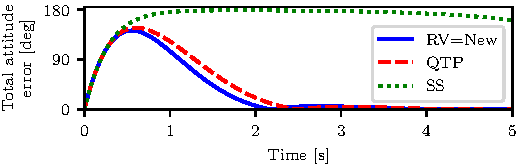
\includegraphics{Figures/fig_case1.pdf}
  \caption{
  来自 \secref{secPerfInitAngVel} 的示例:从大的初始角速度恢复,显示了斜对称控制器的灾难性性能。 
  	`SS' 指的是斜对称控制器方程 \eqref{eqDefInputSS},`RV' 指的是旋转向量控制器方程 \eqref{eqDefInputRotVec},`QTP' 指的是基于四元数的倾斜优先级控制器方程 \eqref{eqDefInputQTP},并且 `New' 指的是提议的控制器方程 \eqref{eqDefInputNew}。
  	基于旋转向量的控制器的行为与新控制器的行为相同。
  }
  \label{figCaseLargeInitVel}
\end{figure}


假设飞行器静止起步,但有一个姿态误差为 $\rho\approx180^\circ$。
从方程 \eqref{eqSkewSymmControllerAxAngle} 可以清楚地看出,由于采用了角度的正弦,斜对称控制器指令的角加速度大约为零。
在飞行中,这本身就是一个安全问题 -- 虽然只要姿态不精确在 $\rho=180^\circ$ 处,最终会收敛到所需的姿态,但这可能需要任意长的时间。
具体而言,当姿态误差超过 $90^\circ$ 时,姿态控制的`刚度'开始\emph{下降}。
在四个控制器中,这是斜对称控制器所独有的。 

为了更生动地说明这一潜在的安全问题,考虑一个初始姿态误差为零的飞行器,但角速度为 $\angVel(0)=\mrb{10.8,0,0}$rad/s。
系统的反应显示在 \figref{figCaseLargeInitVel}。
值得注意的是,所有控制器都能迅速将角速度降为零,但斜对称控制器的姿态误差徘徊在 180$^\circ$ 左右。
基于旋转向量的控制器和所提出的新控制器性能相同,并且略优于基于四元数的推力优先控制器。 

尽管之前已经注意到斜对称控制器收敛缓慢的可能性 \cite{lee2012exponential},但该控制器在文献中仍然很受欢迎(例如文献 \cite{simha2017almost,sreenath2013geometric,rashad2017design})。

\subsection{倾斜优先的优点}
\label{secPerfAdvantageTiltPrior}
\begin{figure}
  \centering
  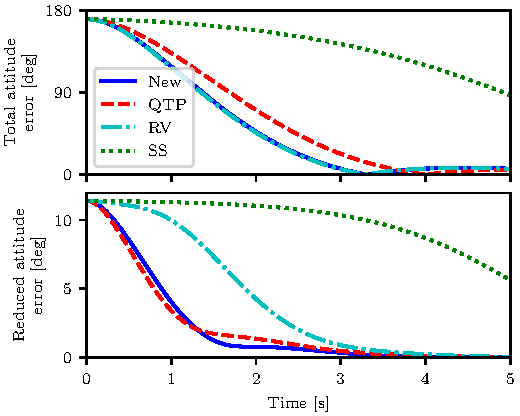
\includegraphics{Figures/fig_case2.pdf}
  \caption{
  来自 \secref{secPerfAdvantageTiltPrior} 的示例:从大的初始偏航误差中恢复,初始倾斜误差较小,显示了拟议的控制器的推力方向的更快速收敛。
  }
  \label{figCaseLargeLargeYaw}
\end{figure}

根据设计,倾斜优先控制器应使飞行器的推力方向更快地收敛到期望的推力方向。
作为这种行为的一个示例,考虑一个从静止开始的飞行器,但围绕轴 $\rotAxis(0)\approx\mrb{0.0995,0,0.995}$ 已旋转 170$^\circ$,因此飞行器有很大的偏航误差,但只有轻微的倾斜误差。
在 \figref{figCaseLargeLargeYaw} 中比较了控制器的性能,可以看出,基于四元数的控制器和拟议的控制器都比基于旋转向量的控制器减少倾斜误差的速度更快得多。
此外,在这种特定情况下,对于总的姿态误差,拟议的控制器的性能实际上与基于旋转向量的控制器没有什么区别,而基于四元数的倾斜优先控制器的性能明显较差。

斜对称控制器的性能再次特别差。
注意,从某种意义上说,这是一个比上一个例子更``友好''的初始条件,因为飞行器现在主要有一个初始偏航误差,理想情况下,这对飞行器的动力学影响应该很小。
此外,由于多旋翼飞机典型的视觉旋转对称性,这种错误在起飞时比较典型(例如,如果操作员错误地放置飞行器)。
此外,偏航误差没有被特别仔细地选择;对于 $10/180\approx5\%$ 的偏航范围,性能不会比图中所示的更好。

\subsection{倾斜优先的缺点}
\label{secPerfDisadvantageTiltPrior}
\begin{figure}
  \centering
  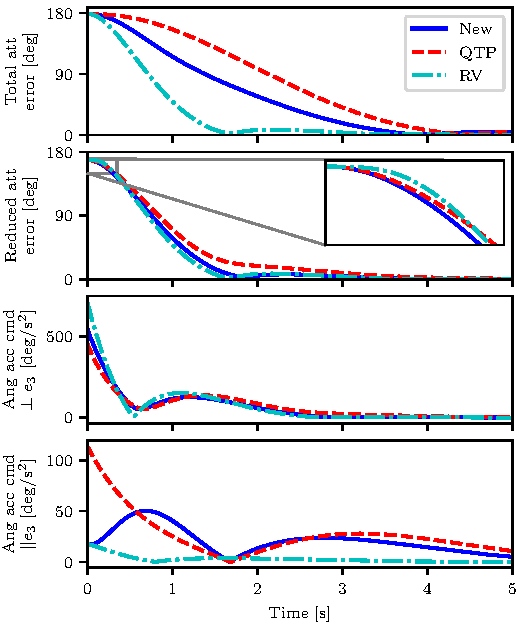
\includegraphics{Figures/fig_case3.pdf}
  \caption{
  来自 \secref{secPerfDisadvantageTiltPrior} 的示例:从大的初始倾斜误差中恢复,初始偏航误差小,显示了基于旋转向量的控制优于拟议的推力优先控制器的例子。
  从上到下:总的姿态误差 $\rotAngle$;减小的姿态误差 $\rotAngleReduced$;垂直于推力方向 $\thrustDir$ 的指令角加速度分量的量值;以及平行于推力方向的指令角加速度分量的量值。
  	插图显示了减小的姿态反应的细节。
  }
  \label{figCaseLargeLargeTilt}
\end{figure}

对于总的姿态误差(而不仅仅是倾斜误差),基于旋转向量的控制通常会优于拟议的控制器,因为它仅直接作用于该误差。
例如,考虑一个围绕轴 $\rotAxis(0)\approx\mrb{0.995,0,0.0995}$的 179$^\circ$ 的初始旋转。
围绕垂直于飞行器推力方向的任意轴线进行的旋转将使飞行器的倾斜误差近乎为零,然而,通过改变旋转轴线的选择,剩余的偏航误差可以是零,也可以大到 $180^\circ$。 

在 \figref{figCaseLargeLargeTilt} 中比较了控制器的性能。
正如预期的那样,基于旋转向量的控制在考虑整体姿态误差时表现最好,在这种情况下,倾斜误差也最终收敛得最快。
基于四元数的控制器和新拟议的倾斜优先控制器在整体姿态误差方面的表现都比较差,但在倾斜角度方面,进行初始化时确实优于基于旋转向量的控制器。
值得注意的是,在初始化阶段,拟议的控制器可以最快地减少`减小的姿态误差'。 

此外,值得注意的是,拟议的控制器在倾斜误差和总的角度误差方面都优于基于四元数的控制器。
此外,它在这样做的同时,还指令降低围绕飞行器推力轴的角加速度峰值,如 \figref{figCaseLargeLargeTilt} 底部所示,尽管总的姿态误差下降得更快。
这种特性在多旋翼飞行器中通常是可取的,因为它们能够围绕 $\baseVec{1}$ 和 $\baseVec{2}$ 产生比推力方向 $\baseVec{3}$ 更大的扭矩,而围绕 $\baseVec{3}$ 的大的角加速度指令可能会迅速导致电机推力的饱和。 



 
\section{实验验证}
\label{secExpValidation}

我们提出两个实验来证明拟议的控制器,同时也是为了强调上一节所讨论的确定的问题并不限于精心构建的数字模拟。
实验使用 Crazyflie 2.0 四轴飞行器进行,在室内运动捕捉空间中运行。
第一个实验演示了一个带着大的初始偏航误差的飞行器起飞。
在第二个实验中,模拟了大的干扰,以演示飞行器从大的初始误差中恢复。

飞行器采用简单的级联控制结构进行控制,其中期望的平动加速度由位置误差上的比例-微分控制器计算, 
\begin{align}
  \translAccDes := -\gainPos \mrb{\pos - \posDes} - \gainVel \dot{\pos}
\end{align}
根据期望的加速度,期望的方向被生成为最小旋转矩阵 $\rotMatDes$ ,对其来说 
\begin{align}
	\translAccDes = \frac{1}{\mass} \rotMatDes \thrustDir \thrustMagDes + \gravity
\end{align}
其中 $\thrustMagDes$ 是期望的推力量值,也是通过上述定义。 

注意,这是一个不复杂的控制结构,但它足以证明拟议的控制法。

\commentOut{
Specifically, in the experiments, the following constants are used:
\begin{align}
  & \gainPos = 2 \mathrm{s}^{-2}
  & \gainVel = 4\sqrt{2}\mathrm{s}^{-1}
\\&\gainAttRed = 167 \mathrm{s}^{-2} 
  &\gainAttYaw = 2 \mathrm{s}^{-1} 
\\&\gainAtt    = \diag{\gainAttRed,\gainAttRed,\gainAttYaw}
  &\gainRates  = \diag{33,33,2} \mathrm{s}^{-1}
\end{align}
}

\begin{figure}
  \centering
  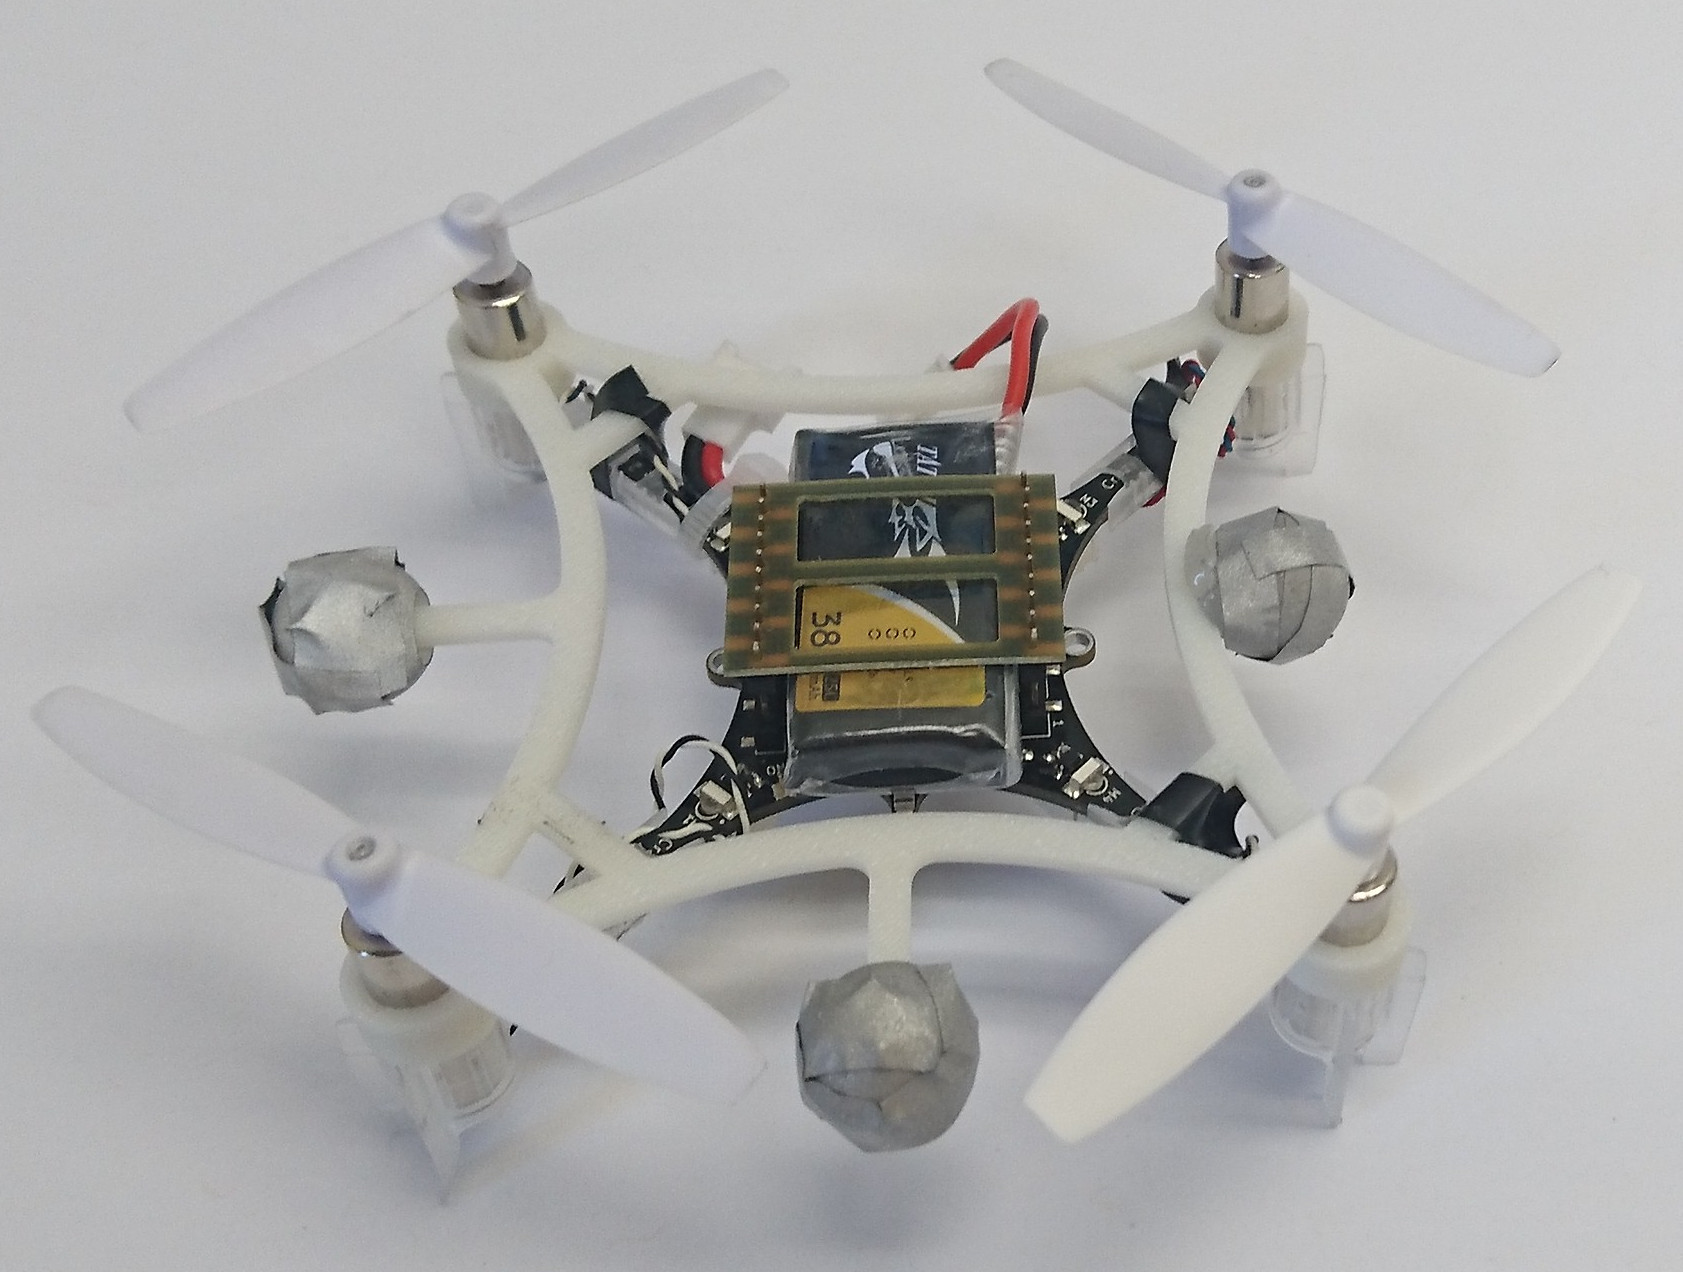
\includegraphics[width=0.7\linewidth]{Figures/quadcopter.jpg}
  \caption{
  实验中使用的四旋翼飞机,从螺旋桨尖到对置螺旋桨尖的尺寸约为 160mm。
  }
  \label{figExpQuad}
\end{figure}

\subsection{起飞时有大的偏航误差}
典型的多旋翼飞机的旋转对称性使得操作者很容易放置一个初始偏航误差较大的多旋翼飞机,这一点在 \figref{figExpQuad} 中可以看到。
为了说明这种误差的实际效果,一个四轴飞行器被命令起飞,并飞到一个高度为 1.5m 的设定点,在离起飞位置大约 0.5m 的水平距离。 
然而,四轴飞行器在初始化时有大的偏航误差(大约 177$^\circ$)。
在 \figref{figExpYaw} 中显示了新控制器和斜对称控制器的五个实验的位置轨迹。 
正如在 \secref{secPerfAdvantageTiltPrior} 中所预期的那样,斜对称控制器的表现非常差,在所有情况下,飞行器在到达目标点之前都会在目标点附近蜿蜒一段距离(如果它没有首先与墙壁相撞的话)。 
拟议的控制器没有表现出这种行为。

\begin{figure}
  \centering
  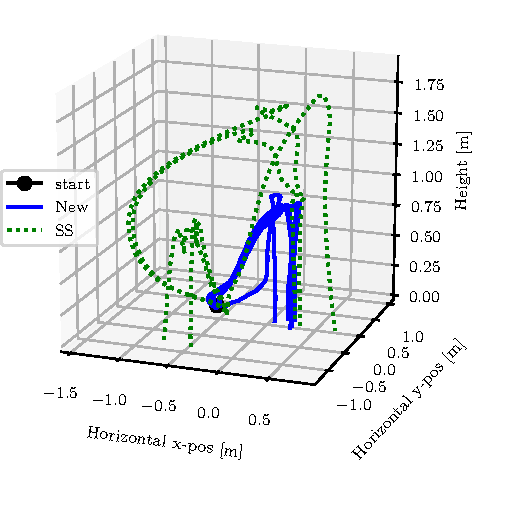
\includegraphics{Figures/Experiments/YawErrTakeoff/fig_traces.pdf}
  \caption{
  四轴飞行器从黑点开始,被命令沿 $x$ 方向水平飞行 0.5m,高度为 1.5m 的位置痕迹(对于多次实验)。
  四轴飞行器开始时有大的偏航误差。
  轨迹的变化是由于系统中的噪声造成的。
  }
  \label{figExpYaw}
\end{figure}

\subsection{从大的初始误差中恢复}
为了证明拟议的控制器在从大的干扰中恢复时的性能,我们进行了一系列的实验,在这些实验中,四旋翼飞机被用户抛到高空,而控制器只在飞行器超过一定的高度阈值时才启动。
这些实验的结果显示在 \figref{figExpLargeDisturbance} 中 -- 从图中可以看出,减小的姿态误差被迅速控制到零,而总的姿态误差可能衰减得更慢。 
这与之前的数值模拟示例的直觉相符。

\begin{figure}
  \centering
  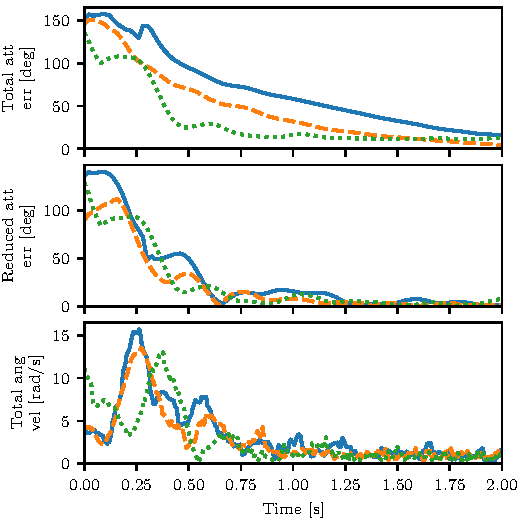
\includegraphics{Figures/Experiments/LargeDisturbances/fig_hists.pdf}
  \caption{
  一个飞行器在被用户扔到空中后,使用拟议的控制器从大的初始干扰中恢复的实验结果。 
  控制动作在时间 0 后立即开始,并且每种线条样式在三个图中标识相同的实验。
  姿态误差由运动捕捉数据估计,角速度由速率陀螺仪测量。
  }
  \label{figExpLargeDisturbance}
\end{figure}
 

\section{\normalfont\bfseries 结论\label{sec:Conclusions}}

本项工作对于基于对偶四元数代数的移动机械臂动力学模型的表示方法,提出了两种策略。第一种是基于递归牛顿-欧拉公式,并使用运动旋量和动力旋量代替自由向量。这种表示方法消除了对运动链进行详尽几何分析的必要性,因为动力旋量和运动旋量是通过高级代数运算传播的。此外,我们的公式适用于任意类型的关节,因为它考虑了任意运动旋量。因此,我们的策略比Miranda等人\cite{MirandadeFarias2019Journal}的工作更一般,他们只考虑具有旋转关节的机械臂。

第二种方法基于高斯最小约束原理,并且它也被制定基于对偶四元数代数所表示的运动旋量和动力旋量的矩阵形式,该策略允许在优化公式中直接加入等式约束。

所提议方法与经典方法的成本比较表明,在乘法和加法次数方面,对偶四元数的使用不会显著增加牛顿-欧拉形式的成本,因为该算法对运动链中的刚体数量具有线性复杂度。然而,使用高斯最小约束原理和对偶四元数代数得到欧拉-拉格朗日模型的成本高于在文献中发现的最佳经典欧拉-拉格朗日递推解。尽管如此,我们的方法远比这些经典的方法更通用。另外,我们没有做出任何努力来优化我们的实现(如果有的话),因为我们目前更感兴趣的是使用对偶四元数代数进行动态建模的理论方面,而不是确保计算效率。在我们目前的MATLAB实现中,dqNE和dqGP平均分别需要 23.17s 和 8.73s 以产生$50$自由度机械臂机器人的关节加速度。在C++实现中,这些值预计将分别减少到 99 ms 和 37 ms 左右 \cite{AdornoDQRobotics2020}。

通过牛顿-欧拉形式获得欧拉-拉格朗日模型需要多次执行该算法。一次执行以获得重力向量,一次执行以获得科里奥利项和离心项的向量,并且对于惯量矩阵 $\mymatrix M$ 的每一行都执行一次。对于一个$50$自由度机械臂的机器人,每个模拟步骤执行 $52$ 次dqNE。然而,对于控制应用,我们通常是对寻找关节扭矩感兴趣,它只需要执行一次dqNE以产生每个控制输入。因此,使用dqNE计算$50$自由度机械臂机器人的关节扭矩,在C++实现中,执行时间预计将减少 $52$ 倍,从大约 99~ms 减少到 1.9~ms。

最后,对于三种不同机器人,我们通过提议的策略获取的关节加速度,与从 ${\text{V-REP PRO EDU V3.6.2}}$ (一个真实的模拟器)中获取的值进行了比较。结果表明,我们所有的方法对于固定基座串联机械臂和移动机械臂都是精确的。

未来的工作重点是将对偶四元数牛顿-欧拉算法推广到非串联多体系统(如仿人系统),以及动力旋量控制策略中。对于使用高斯最小约束原理和对偶四元数代数获得的欧拉-拉格朗日模型,未来的工作将集中于在优化表示方法中运用不等式约束。


\section*{Acknowledgements}
This research was supported by funding from the Powley foundation.
We also thank Koushil Sreenath and Dario Brescianini for their valuable inputs. 

\bibliographystyle{plainnat}
\bibliography{bibliography}

%\bibliographystyle{IEEEtran}
%\bibliography{bibliography}

\end{document}
